\documentclass[abstract=on,9pt,twocolumn]{scrartcl}

\usepackage[paper=a4paper,top=2cm,left=1.5cm,right=1.5cm,bottom=2cm,foot=1cm]{geometry}
\usepackage{ucs}
\usepackage[utf8x]{inputenc}
\usepackage[T1]{fontenc}
\usepackage[english]{babel}
\usepackage{relsize}%	relative font sizes
\usepackage[retainorgcmds]{IEEEtrantools}%	IEEEeqnarray
\setlength{\IEEEnormaljot}{4\IEEEnormaljot}
\usepackage{graphicx}
\usepackage{epstopdf}
\usepackage{indentfirst}
\usepackage{hyperref}
%\usepackage{cleveref}
%\usepackage[noabbrev]{cleveref}
\usepackage{listings}
\usepackage{color}

\lstset{
	language=C++,
	basicstyle=\ttfamily,
	showspaces=false,
	showtabs=false,
	tabsize=3,
	captionpos=b,
	breaklines=true,
	breakatwhitespace=true
}

%%%%%%%%%%%%%%%%
%  title page  %
%%%%%%%%%%%%%%%%

\titlehead{University of Minho \hfill Master's Degree in Informatics Engineering\\	Department of Informatics \hfill Parallel and Distributed Computing}
\title{Parallel Radix Sort}
\subtitle{OpenMP and MPI analysis and comparison}
\author{Miguel Palhas \hfill--- \texttt{\smaller pg19808@alunos.uminho.pt}}
\date{Braga, May 2012}
\subject{Parallel Computing Paradigms}


%%%%%%%%%%%
%  Hacks  %
%%%%%%%%%%%

%	Paragraph (title) with linebreak
\newcommand{\paragraphh}[1]{\paragraph{#1\hfill}\hfill

}

\begin{document}
	\maketitle

	\begin{abstract}

	This paper describes the implementation, testing, and performance analysis of a parallel sorting algorithm, specifically Radix Sort. At first an initial, sequential implementation was created. A shared memory implementation followed, using OpenMP. Finally a distributed memory approach was also tried, with MPI, where the problem of load balancing was also taken into account. This resulted in two different MPI implementations, one with load balacing, and one without it.
\end{abstract}
		% Abstract
	\section{Introduction}
\label{sec:intro}
% why are we doing this report
% TODO

	Intro here
		% Introduction
	\section{The Algorithm}
\label{sec:radix}

Radix Sort is a non-comparative sorting algorithm that works on integer or string keys. The ordering is done by grouping keys into buckets, according to their individual digits.\\

There are two variants of the algorithm. The \emph{Least Significant Digit Radix Sort} which starts by grouping keys based on their least significant digit. After each key is sent to their respective bucket, the buckets are concatenated orderly. At this point the keys will be ordered up to the digit upon which the step was made. After iterating through all the digits, the keys are ordered. The \emph{Most Significant Digit Radix Sort} uses a different approach, and is recursive in nature. Starting on the most significant digit, keys are grouped to their buckets. However, instead of merging all buckets after this step, a recursive step is taken, ordering each bucket internally based on the next digit.\\

This report will focus only on the first version, since it's an iterative, simple method, instead of a recursive one, and because of that, it's parallelization is not only easier to implement, but probably allows for better load balance.\\


\subsection{How it works}
\label{subsec:how_it_works}

Consider the following list of integers:

\begin{IEEEeqnarray*}{C}
	[170, 45, 75, 90, 802, 24, 2, 66]
\end{IEEEeqnarray*}

In the first iteration, the least significant digit is considered. After sending each key into the correct bucket, the result is the following:

\begin{IEEEeqnarray*}{C}
	0: [170, 90],	\\
	2: [2], 4: [24]	\\
	5: [45, 75]		\\
	6: [66]
\end{IEEEeqnarray*}

And after merging all buckets:

$$ [170, 90, 2, 24, 45, 75, 66] $$
		% Radix explanation
	\section{Sequential Implementation}
\label{sec:seq}

The initial implementation is straight-forward, following the explanation given on \autoref{subsec:how_it_works}. There are some differences however. Instead of base-10 digits, groups of bits were used. Each digit will consist of a group of bits, allowing for better performance (by using bitwise operators), and also to give the possibility of easily varying the amount of bits per digit.

With a smaller amount of bits per digit, less buckets will be used (number of buckets is equal to $2^g$, where $g$ is the number of bits). Consequentely, more iterations will be necessary. On the other hand, a bigger value of $g$ will require more buckets, increasing the fragmentation of the data and memory overhead.
			% Sequential implementation
	\section{OpenMP Implementation}
\label{sec:omp}

For the OpenMP implementation used, 3 steps are required in each iteration:

\begin{enumerate}
	\item Bucket Fill
	\begin{itemize}
		\item[-] For $P$ threads and $B$ buckets, each thread will handle $B/P$ buckets
		\item[-] Each thread iterates entire array, inserting only on its own buckets
	\end{itemize}

	\item Master thread computes offset for each bucket on the result array

	\item Each thread copies its buckets to global array
\end{enumerate}

Given that radix sort is a non-comparative sorting algorithm, and it consists mostly on memory operations, it can be easily seen that it is completely memory bound. Because of that, no good results should be expected from this shared-memory implementation. Since memory is already the bottleneck, no benefit is taken from asking more from it.
			% OpenMP implementation
	\section{MPI Implementation}
\label{sec:mpi}

The MPI version follows a completely different strategy. This was entirely based on the article [\cite{paper}].

For this implementation, it is assumed that each process owns a partition of the array, and that all partitions are equal in size. Also, like the OpenMP version, each bucket is assigned to a single process. So for $B$ buckets, a maximum of $P$ processes should be used, otherwise no significant improvements would happen.

The general workflow for each iteration is:

\begin{enumerate}
	\item \textbf{Local Bucket fill}. Each process creates a list of buckets indexing its local partition. An auxiliary array of size $B$ is also created, containing the size of each local bucket.

	\item \textbf{\emph{all-to-all} transpose}. Each process will now need information about the size buckets that are assigned to them. For instance, if process 0 is handling bucket 0, then all other processes will be required to inform him about the size of their local bucket 0. The global bucket 0 will have a size equal to the sum of each local one. This operation is more clearly shown in \autoref{fig:mpi}

	\item \textbf{Communication}. Knowing how many elements each bucket will have, every process will now send the keys to the apropriate destinations
\end{enumerate}

\begin{figure}[!htpb]
	\begin{center}
		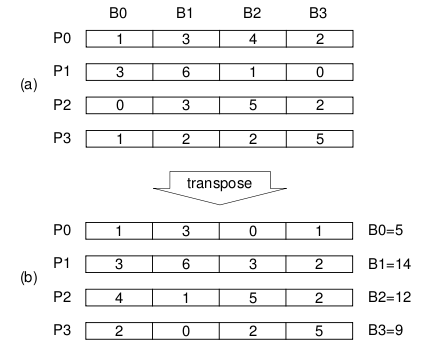
\includegraphics[width=0.45\textwidth]{images/mpi}
	\end{center}
	\caption{\emph{all-to-all} transpose operation. (a) shows the local bucket sizes in each proc. With eack bucket being assigned to one process, the transpose of this, being shown in (b) ilustrates the wanted result}
	\label{fig:mpi}
\end{figure}

Besides ilustrating how the transpose operation works, \autoref{fig:mpi} also happens to expose the problem with this implementation, which is load balancing. For example, after the iteration shown, P0 will have 5 elements on its local partition, and P1 will have 14. The next iteration will give completely different values for each process, since each iteration is based on an entirely different digit. Not only is the amount of elements per process completely unbalanced, the communication is also a problem.
			% MPI implementation
	\section{MPI Load Balancing}
\label{sec:mpi_bal}

To solve the load balance problem, a different strategy is sugested in \cite{paper} to implement the distribution of keys across each processor at the end of each iteration.

The original approach assigns each bucket to one processor. Since bucket have a wide range of sizes, this creates a big inbalance in key distribution. The approach used changes the division process. Each process is first required to receive all information about local bucket counts of all other processors, effectively getting information about how many elements are in every bucket of every process. With this information, a division can be mande across all this information, to equally distribute keys across each processor. \autoref{fig:mpi} illustrates this approach.

\begin{figure}[!htpb]
	\begin{center}
		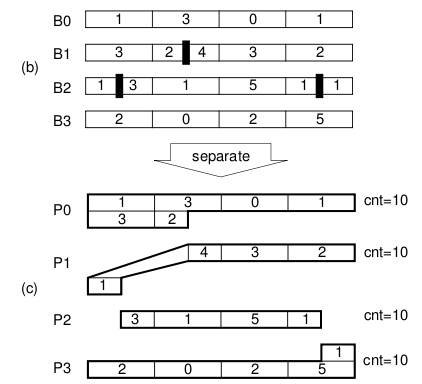
\includegraphics[width=0.45\textwidth]{images/mpi_bal}
	\end{center}
	\caption{An illustration of the load balancing strategy used on the second MPI implementation}
	\label{fig:mpi}
\end{figure}


		% MPI Load Balance
	\section{Communication}
\label{sec:comm}

Each of the two MPI implementations consists of two communication steps, but they have different dimensions in each one.

\begin{itemize}
	\item \textbf{Bucket count communication}. In the first implementation, each process has to send each of their local bucket sizes to a single process. So for the complete matrix of all bucket sizes (this matrix has size $P \times B$) each element requires a single Send/Receive. This makes the complexity for this step $\Theta(P \cdot B)$
		With the addition of load balance control, this entire matrix has to be sent to every processor, making complexity becomes $\Theta(P^2 \cdot B)$. Although this complexity is higher for the version that should provide the best results, this is because the main overhead is not in the bucket size communication, but in the communication of the elements themselves. The number of buckets is usually really small (only 256 buckets for $g=8$), and the input can consist in millions of elements, this difference is clear.

	\item \textbf{Keys communication}. Each process has to send their local keys to the apropriate destination. So for $N$ keys, the complexity of communication becomes $O(N)$. Notice that this is $O$ notation and not $\Theta$ because some of the keys may already be in the appropriate process, requiring only a local copy in memory. The difference is in the balance of the keys. For the first version, the number of keys that a single process sends or receives can be anything between 0 and $N$, and it may happen that the weight of communication will be only in a subset of all processes, increasing communication delay. But in the second implementation, each process is garanteed to send exactly $N/P$ keys and receive that same amount back from other processes. This may have a huge impact in communication delay, and consequentely, in the overall performance of the algorithm.

\end{itemize}

Also note that this analysis refers only to a single iteration of radix sort. Every iteration has the same complexity, so the overall complexity will be equal to the one of a single iteration, multiplied by the number of iterations.
			% Communication details
	% TODO add stuff here
	
	\section{Conclusion}

\begin{frame}
	\frametitle{Conclusion}

\begin{itemize}\itemsep=10pt
		\item Radix sort is completely memory bound
		\begin{itemize}
			\item[-] Easily confirmed by observing the C++ code
			\item[-] OpenMP not homogeneous, gives bad results
		\end{itemize}


		\item MPI shows speedups for larger input sizes, but nothing amazing
		\begin{itemize}
			\item[-] Implementation problems
			\item[-] Source paper \footnote{\emph{``Load Balanced Parallel Radix Sort''}, Andrew Sohn and Yuetsu Kodama} claims 40-fold speedups with 64 processors
		\end{itemize}

	\item Load Balanced strategy proved useful for bigger inputs
		\begin{itemize}
			\item[-] But technical problems prevented further analysis
		\end{itemize}

	\end{itemize}

\end{frame}
	% Conclusion

	\begin{thebibliography}{12345}
		\bibitem[sohn\_load]{paper}
			Sohn, A. and Kodama, Y.	\\
			\textit{Load balanced parallel radix sort}	\\
		    Proceedings of the 12th international conference on Supercomputing	\\
	\end{thebibliography}

\end{document}
